	%Template by Mark Jervelund - D1 - 2015 - mjerv15@student.sdu.dk

\documentclass[a4paper,10pt,titlepage]{report}

\usepackage[utf8]{inputenc}
\usepackage[T1]{fontenc}
\usepackage[english]{babel}
\usepackage{amssymb}
\usepackage{amsmath}
\usepackage{amsthm}
\usepackage{graphicx}
\usepackage{fancyhdr}
\usepackage{lastpage}
\usepackage{listings}
\usepackage{algorithm}
\usepackage{algpseudocode}
\usepackage[document]{ragged2e}
\usepackage[margin=1in]{geometry}
\usepackage{color}
\usepackage{datenumber}
\usepackage{venndiagram}
\usepackage{chngcntr}
\setdatetoday
\addtocounter{datenumber}{0} %date for dilierry standard is today
\setdatebynumber{\thedatenumber}
\date{}
\setcounter{secnumdepth}{0}
\pagestyle{fancy}
\fancyhf{}

\newcommand{\Z}{\mathbb{Z}}
\lhead{Database Management Systems (DM556))}
\rhead{Mark Jervelund (Mjerv15) Troels B. Petersen (trpet15)}
\rfoot{Page  \thepage \, of \pageref{LastPage}}
\counterwithin*{equation}{section}

\lstset{
  numbers=left,
  stepnumber=5,    
  firstnumber=1,
  numberfirstline=true
  frame=single,
  breaklines=true,
  postbreak=\raisebox{0ex}[0ex][0ex]{\ensuremath{\color{red}\hookrightarrow\space}}
}

\begin{document}
\begin{titlepage}
\centering
    \vspace*{9\baselineskip}
    \huge
    \bfseries
    Project 3\\
    
    \normalfont 
	\huge    
    Database Management Systems (DM556)  \\[4\baselineskip]
    \normalfont
	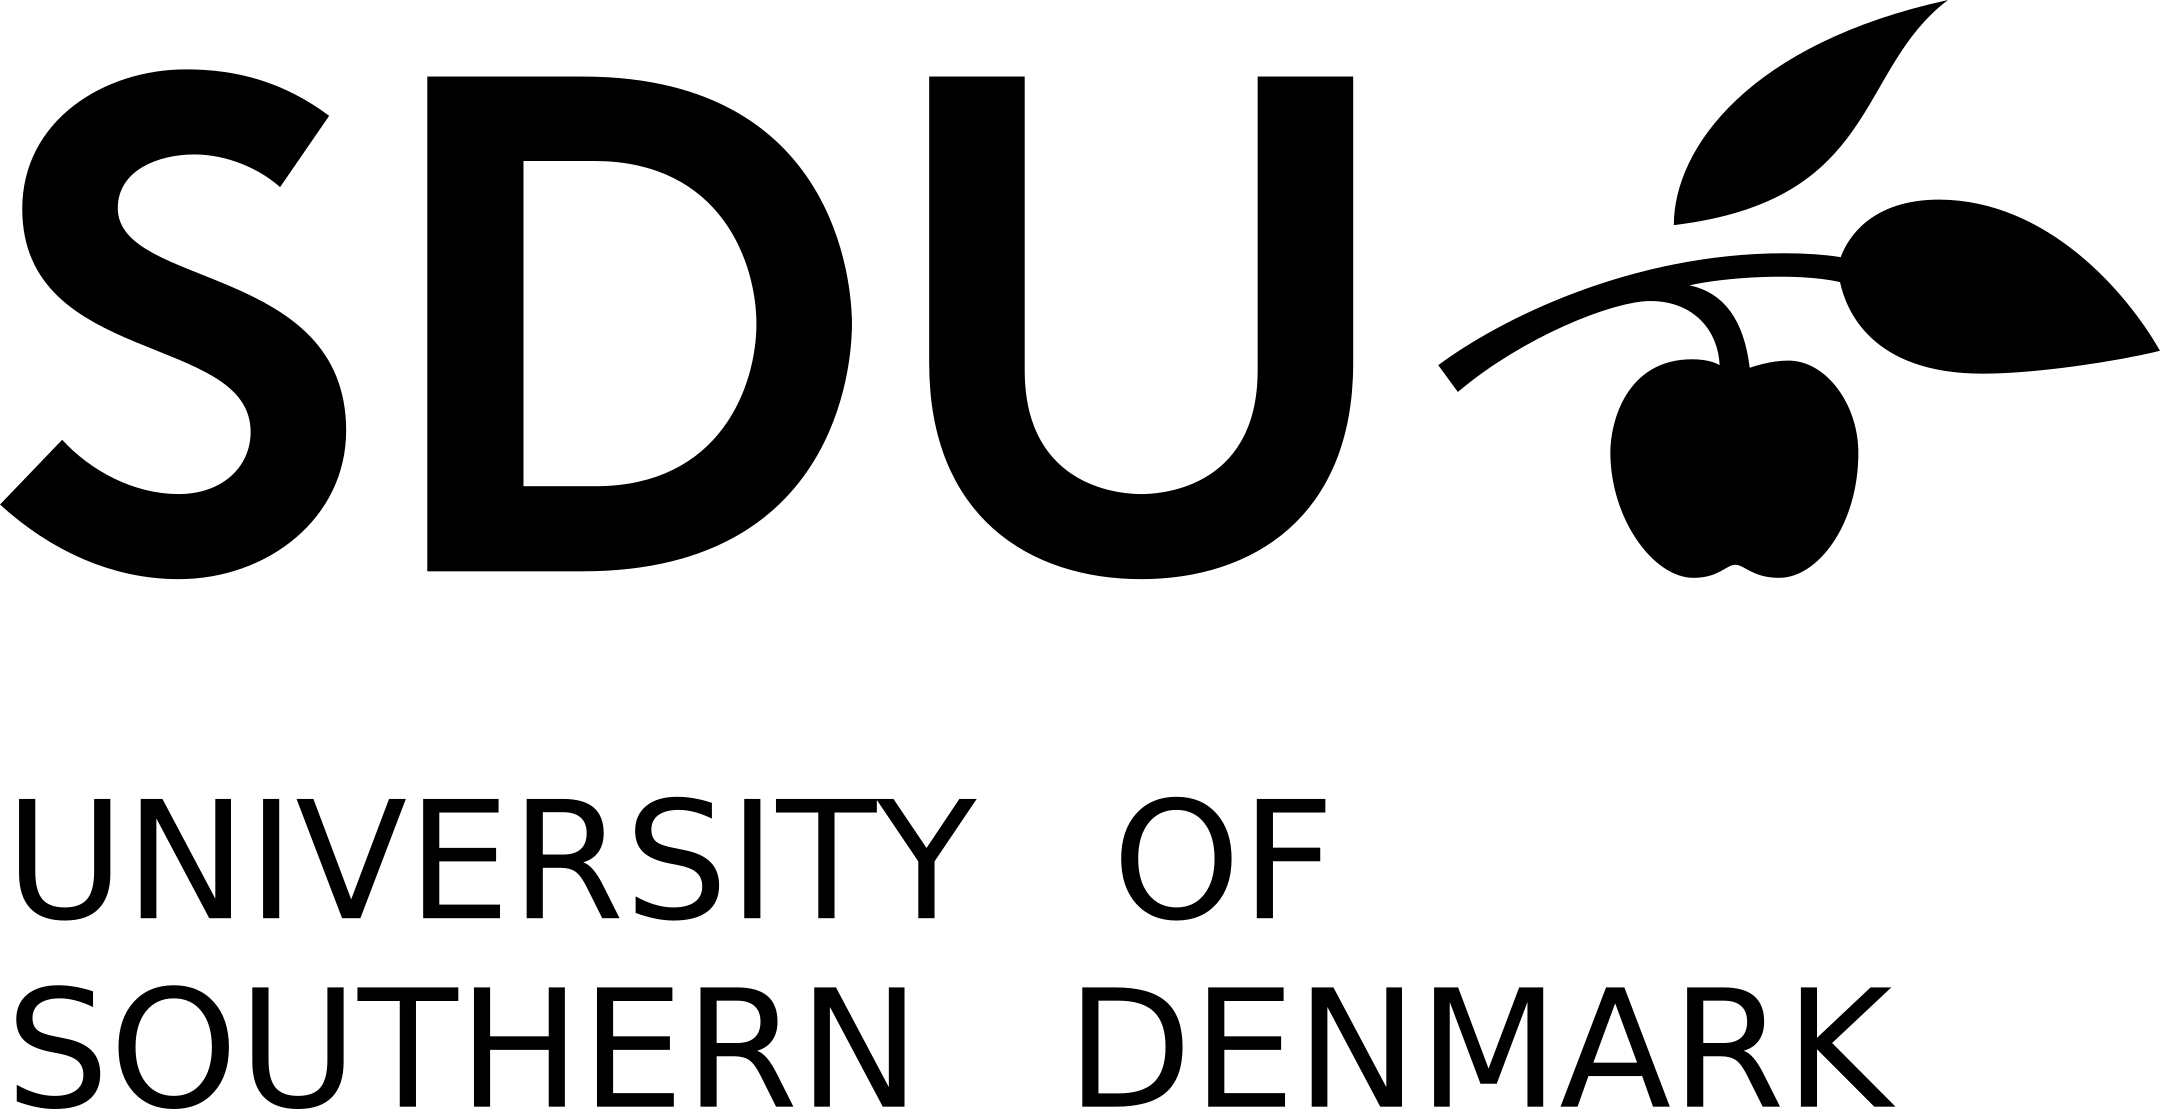
\includegraphics[scale=1.5]{SDU_Logo}
    \vfill\
    Group 2\\
    Mark Jervelund (Mjerv15)    Troels B. Petersen (trpet15)
    \vspace{5mm}
    IMADA \\
    \textbf{\datedate} \\[2\baselineskip]
\end{titlepage}
%\renewcommand{\thepage}{\roman{page}}% Roman numerals for page counter
%\tableofcontents

%\newpage
\setcounter{page}{1}
\renewcommand{\thepage}{\arabic{page}}

\lstset{language=Java}          % Set your language (you can change the language for each code-block optionally)
\section{Overall Status}
The group managed to complete the tasks and therefore the project is considered complete, however, due to human error we thought the deadline was at 23:30 and not at 12:00, so we agreed with Yongluan ZHOU to upload what we had at 12 and email the rest within the day.
\section{Division of Labor}
The group worked on the project either sitting together at the university or at home remotely working together and splitting tasks when possible. A lot of the time was spent understanding how to implement a solution. However, due to several other group projects going on simultaneously, 
\section{Specification}
In the third assignment of the course we are tasked with implementing a basic query optimizer for select and 2 other elective assignments.\\

For the elective assignment i choose to implement update and delete and Pushing down predicates \\


\subsection{Select}
Implement the basic query optimizer for the select class, you most call the Query check class to validate input. the default plan is to use file scans and simple joins for all tables, and a selection for each conjunct, and have one projection at the root of the tree.

\subsection{delete \& update }

implement the two query types delete and update.

\subsection{Pushing down predicates}
If possible the selection should push down predicates in the tree if possible.



%\subsection{Design}
%
%Flushpages was implementing using Flushpage as they're almost %doing the same and this reduces the amount of dubplicate code. 

\section{Implementation}
The files \textsf{Select.java}, \textsf{Update.java} and \textsf{Delete.java} were implemented to provide the wanted functionality.

\subsection{Select.java}
Select has implemented four functions, one of which is the executer \textsf{execute()} and the constructor \textsf{Select(AST\_Select)} that takes the AST\_Select-object as input. First it is checked whether or not the current tree is an EXPLAIN statement. Then it starts running \textsf{parser(AST\_Select)}.
\vspace{5mm}
\\
\textsf{parser(AST\_Select)} rationalizes the statement, so it makes sense for a computer. It does so, by saving the predicates, tables and columns separately. It then combines(joins) all the tables into one large schema. Afterwards it is checked whether the all the coloumns are present in the new schema. If they are not, the \textsf{QueryCheck.columnExists(...)} will throw an exception.\\ \vspace{5mm)
Very similar is the last part of the function, where \textsf{QueryCheck.predicates} will also throw an exception, if the predicate is illegal and doesn't fit with the tables and columns.
\\
\vspace{5mm}
The \textsf{optimizer()} What happens in the optimizer is that the Tree is optimized so that it performs as few operations as possible
\\
\textsf{execute()} simply executes based on the \textsf{isExplain} boolean. If \textsf{isExplain} is false, it tells how many rows were affected.

\subsection{Delete.java}
The \textsf{Delete()} function deletes records based on the \textsf{AST\_Delete} object. It starts by getting the table that has to be deleted and then checks that it exists. It also gets the predicates, and checks that these are valid. If any of these is illegal, it throws a \textsf{QueryException}.
\\
\textsf{execute()} is where the actual deletion takes place. Here it gets the tables and starts deleting records based on the predicates. It finds the records using keys corresponding to each record, for use in the hashbased database. In the end it reports the amount of records that were affected (deleted).

\subsection{Update.java}
The update Function updates records where a condition is met. what happens in the Update function call is that all the fields, values and predicates are checked for validity.

The update itself happends in the \textsf{execute()}  Here it gets the tables and starts updating records based on the predicates. It finds the records using keys corresponding to each record, for use in the hashbased database. In the end it reports the amount of records that were affected.


%lstinputlisting[firstnumber=111,firstline=111,lastline=120,frame=single]{../DM556-project2/relop/MergeJoin.java}
qfqfqfasqfqfqfqfadqrqrqrqrqfqfqfasdqrqrqrqrqfqfqfqfaqfqfqfas
\subsection{Testing}

\subsection{Select}
\begin{lstlisting}
MSQL> SELECT name,depname FROM Emp, Works,Dept WHERE id = eid AND depid = did;

name                                              depname                                           
----------------------------------------------------------------------------------------------------
Yongluan                                          IMADA                                             
Yongluan                                          ADMINISTRATION                                    
Jacob                                             IMADA                                             
Claus                                             ADMINISTRATION                                    
4 rows affected.
\end{lstlisting}

\subsection{Update}
\subsubsection{Starting point}
\begin{lstlisting}
name                                              id        age       
----------------------------------------------------------------------
Yongluan                                          1         28        
Jacob                                             2         32        
Claus                                             3         42       
\end{lstlisting}
\subsubsection{After update}
\begin{lstlisting}
MSQL> update emp set age = 42 where id = 2;
1 rows affected.
MSQL> select * from emp;

name                                              id        age       
----------------------------------------------------------------------
Yongluan                                          1         28        
Jacob                                             2         42        
Claus                                             3         42        
3 rows affected.
\end{lstlisting}

\subsection{Delete}
\subsubsection{Starting point}
\begin{lstlisting}
MSQL> select * from emp;
name                                              id        age       
----------------------------------------------------------------------
Yongluan                                          1         28        
Jacob                                             2         42        
Claus                                             3         42        
3 rows affected.
\end{lstlisting}
\subsubsection{After update}

\begin{lstlisting}
MSQL> delete from Emp where id = 3;
1 rows affected.
MSQL> select * from emp;
name                                              id        age       
----------------------------------------------------------------------
Yongluan                                          1         28        
Jacob                                             2         42     
2 rows affected.  
\end{lstlisting}

\section{Appendix}
Select.java
\lstinputlisting[frame=single]{..//DM532-project3/query/Select.java}

Delete.java
\lstinputlisting[frame=single]{..//DM532-project3/query/Delete.java}

Update.java
\lstinputlisting[frame=single]{..//DM532-project3/query/Update.java}


\end{document}
